\chapter{Analisis}
\label{chap:analisis}
Bab ini akan membahas analisis-analisis yang dilakukan dalam pengembangan perangkat lunak KIRI. Pada bab ini akan terdapat dua subbab utama, yang pertama, yaitu analisis sistem kini yang akan membahas kelas-kelas yang terdapat pada sistem backend KIRI bernama NewMenjangan. Kemudian yang kedua, yaitu analisis sistem usulan yang akan membahas usulan yang akan dilakukan dalam pengembangan KIRI, seperti implementasi \textit{strategy pattern} serta implementasi algoritma Floyd-Warshall dan A-Star.
\section{Analisis Sistem Kini}
\label{sec:sistemkini}
Analisis akan dilakukan terhadap sistem dari perangkat lunak KIRI yang bernama NewMenjangan. Sistem ini bertanggung jawab untuk menangani berbagai fungsi \textit{backend} yang mendukung layanan utama KIRI, termasuk pengolahan data, komunikasi dengan komponen lain, dan pengelolaan algoritma terkait penelusuran rute. Gambar \ref{fig:strukturkelas}, merupakan struktur kelas saat ini dari aplikasi KIRI yang digambarkan dalam diagram kelas. Saat ini, algoritma yang diterapkan adalah algoritma Dijkstra, yang digunakan untuk melakukan perhitungan dalam pencarian jalur terpendek dalam graf berbobot. Analisis ini mencakup tinjauan menyeluruh terhadap struktur kelas NewMenjangan dan juga pemodelan graf pada perangkat lunak KIRI.
\begin{figure}[h] 
    \centering  
    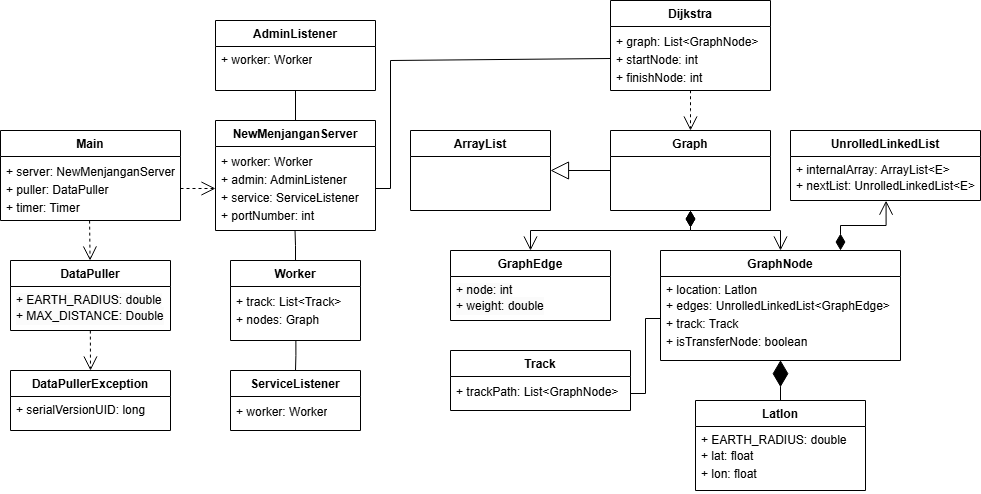
\includegraphics[width=0.9\textwidth]{class-diagram}  
    \caption{Struktur Kelas NewMenjangan}
    \label{fig:strukturkelas} 
\end{figure}

\subsection{Analisis Kelas}
Pada bagian ini, akan dilakukan analisis terhadap struktur kelas yang membentuk sistem \textit{backend} NewMenjangan. Analisis ini bertujuan untuk memahami peran dan hubungan antar kelas dalam sistem, termasuk bagaimana kelas-kelas tersebut berinteraksi untuk menangani pencarian rute menggunakan algoritma Dijkstra. Setiap kelas dalam diagram pada Gambar \ref{fig:strukturkelas} akan dianalisis berdasarkan fungsinya dalam sistem.

\subsubsection{Main.java}
Kelas ini berfungsi sebagai pusat kendali dari \textit{backend} KIRI. Melalui kelas ini, server bisa dijalankan, diperiksa statusnya, dimatikan, dan juga mengolah data. Pada kelas ini, terdapat 5 konstanta dan 5 atribut. Selain itu, terdapat \textit{method - method} diimplementasikan yang memiliki penjelasan sebagai berikut:
\begin{itemize}
    \item \textbf{Konstanta}
    \begin{itemize}
        \item \texttt{TRACKS\_CONF}, \texttt{MYSQL\_PROPERTIES}, dan \texttt{MJNSERVE\_PROPERTIES}
        \\ Konstanta tersebut digunakan untuk mengarahkan pada file konfigurasi yang diperlukan.
        \item \texttt{LOGGING\_PROPERTIES} dan \texttt{NEWMJNSERVE\_LOG}
        \\ Konstanta tersebut digunakan untuk mengatur lokasi konfigurasi \textit{logging} dan \textit{file log}.
    \end{itemize}

    \item \textbf{Atribut}
    \begin{itemize}
        \item \texttt{server}, \texttt{puller}, dan \texttt{timer}
        \\ Atribut-atribut tersebut digunakan untuk mengelola server, menarik data, dan menjalankan tugas terjadwal.
        \item \texttt{portNumber}
        \\ Atribut ini berfungsi untuk menetapkan \textit{port default} yang digunakan oleh server.
        \item \texttt{homeDirectory}
        \\ Atribut ini digunakan untuk menjadi direktori utama yang diambil dari variabel lingkungan \texttt{NEWMJNSERVE\_HOME}, yang diperlukan agar aplikasi berjalan.
    \end{itemize}

    \item \textbf{Method}
    \begin{itemize}
        \item \texttt{main(String[] args)}
        \\ \textit{Method} ini dirancang untuk memproses argumen yang diterima guna memeriksa status server atau menghentikannya. Ketika argumen \texttt{-c} diberikan, fungsi \texttt{sendCheckStatus} akan dipanggil untuk memastikan bahwa server sedang berjalan. Sebaliknya, jika argumen \texttt{-s} diberikan, fungsi \texttt{sendShutdown} akan bertugas mematikan server. Sebelum proses lebih lanjut dilakukan, program memeriksa apakah variabel lingkungan \texttt{NEWMJNSERVE\_HOME} telah diatur. Jika tidak, aplikasi akan segera dihentikan. Setelah inisialisasi konfigurasi \textit{logging} selesai, fungsi \texttt{pullData} dijalankan untuk menarik data yang diperlukan. Server kemudian dimulai melalui pemanggilan metode \texttt{server.start()}, dan sebuah \texttt{ShutdownHook} disertakan untuk memastikan penghentian server dilakukan dengan aman.
\newpage
        \item \texttt{sendCheckStatus(int portNumber)} dan \texttt{sendShutdown(int portNumber)}
        \\ Keduanya menggunakan koneksi HTTP untuk mengirim permintaan ke server. \textit{Method} \texttt{sendCheckStatus} berfungsi untuk mengecek status server, sementara \textit{method} \texttt{sendShutdown} mengirim permintaan untuk mematikan server.

        \item \texttt{pullData()}
        \\ \textit{Method} ini bertugas untuk menarik data dari sumber SQL dan sumber eksternal lainnya. Jika terjadi perubahan pada file konfigurasi \texttt{tracks.conf}, data yang ada akan ditimpa dengan data baru yang diperbarui. Selain itu, proses pembaruan ini akan dicatat dalam log untuk pemantauan perubahan data yang terjadi. \textit{Method} akan mengembalikan nilai \texttt{true} apabila penarikan data berhasil dan \texttt{false} apabila gagal.

        \item \texttt{fileEquals(File file1, File file2)}
        \\ \textit{Method} ini dirancang untuk membandingkan dua file secara biner untuk menentukan kesamaan di antara keduanya. Jika kedua file memiliki panjang yang berbeda, maka file tersebut secara otomatis dianggap tidak identik. Selain itu, jika ditemukan perbedaan byte pada posisi tertentu selama proses pembandingan, posisi perbedaan tersebut akan dicatat dalam log. \textit{Method} akan mengembalikan nilai \texttt{true} apabila file \textit{identical} dan \texttt{false} apabila tidak \textit{identical}.
        
    \end{itemize}
\end{itemize}

\subsubsection{AdminListener}
Kelas ini berfungsi sebagai \textit{handler} HTTP khusus yang menerima perintah-perintah administratif untuk mengelola server \textit{backend} KIRI. Kelas ini memungkinkan aplikasi \textit{backend} menerima dan menjalankan perintah administrasi dari localhost melalui HTTP. Pada kelas ini, terdapat 1 atribut diinisialisasikan serta \textit{method-method} diimplementasikan yang memiliki penjelasan sebagai berikut:
\begin{itemize}
    \item \textbf{Atribut}
    \begin{itemize}
        \item \texttt{worker}
        \\ Variabel ini bertipe \texttt{Worker} yang merupakan sebuah kelas. \texttt{worker} ini diperlukan untuk menjalankan perintah-perintah tertentu, seperti \texttt{tracksinfo}.
    \end{itemize}
    
    \item \textbf{Method}
    \begin{itemize}
        \item \texttt{handle(String target, Request baseRequest, HttpServletRequest request, \\HttpServletResponse response)}
        \\ \textit{Method} ini mengimplementasikan penanganan permintaan HTTP dengan memanfaatkan kelas \texttt{AbstractHandler} dari \textit{library} Jetty. Ketika sebuah permintaan HTTP diterima, \textit{method} ini akan melakukan beberapa langkah. Pertama, sumber permintaan diperiksa untuk memastikan bahwa hanya permintaan dari localhost yang diterima. Selanjutnya, \textit{method} ini memproses parameter query string dari URL untuk mengidentifikasi perintah yang diminta. Dengan pendekatan ini, setiap permintaan dapat diproses sesuai dengan parameter yang dikirimkan.
        \\ \textit{Method} ini mendukung berbagai jenis perintah yang dapat diterima melalui permintaan HTTP. Salah satu perintah adalah \texttt{forceshutdown}, yang berfungsi untuk menghentikan server setelah jeda satu detik dengan menjalankan \texttt{System.exit(0)} dalam sebuah \textit{thread} baru. Perintah lain, yaitu \texttt{tracksinfo}, akan mengembalikan informasi mengenai jalur jika \texttt{worker} telah diinisialisasi, menggunakan metode \texttt{worker.printTracksInfo()}. Selain itu, perintah ping akan mengembalikan string "pong" untuk memverifikasi bahwa server sedang aktif. Apabila perintah yang diterima tidak valid atau tidak dikenali, metode ini akan mengembalikan status dan pesan kesalahan yang sesuai.
        \\ Pengaturan status dan pesan respons dilakukan berdasarkan hasil dari setiap perintah yang diproses. Jika perintah berhasil dijalankan, status \texttt{HttpStatus.OK\_200} akan dikembalikan. Jika permintaan berasal dari alamat selain localhost, status yang dikembalikan adalah \texttt{HttpStatus.FORBIDDEN\_403}. Permintaan yang tidak mencantumkan perintah akan menerima status \texttt{HttpStatus.BAD\_REQUEST\_400}, sedangkan jika worker belum siap, status \texttt{HttpStatus.SERVICE\_UNAVAILABLE\_503} akan diberikan.
    \end{itemize}
\end{itemize}

\subsubsection{NewMenjanganServer}
Kelas ini berfungsi untuk menginisialisasi dan menjalankan server HTTP yang mendengarkan permintaan pada \textit{backend} KIRI. Server ini menggunakan \textit{library} Jetty untuk menangani permintaan HTTP. Pada kelas ini, terdapat 1 konstanta dan 6 atribut. Selain itu, terdapat sebuah konstruktor dan \textit{method-method} diimplementasikan yang memiliki penjelasan sebagai berikut:
\begin{itemize}
    \item \textbf{Konstanta}
    \begin{itemize}
        \item \texttt{DEFAULT\_PORT\_NUMBER}
        \\ Merupakan nomor port \textit{default} yang digunakan jika tidak ada port yang ditentukan.
    \end{itemize}

    \item \textbf{Atribut}
    \begin{itemize}
        \item \texttt{worker}
        \\ Merupakan instance dari kelas \texttt{Worker}.
        \item \texttt{admin}
        \\ Merupakan instance dari kelas \texttt{AdminListener}.
        \item \texttt{service}
        \\ Merupakan instance dari kelas \texttt{ServiceListener}.
        \item \texttt{httpServer}
        \\ Merupakan server Jetty yang akan mendengarkan permintaan HTTP.
        \item \texttt{portNumber}
        \\ Berfungsi untuk menyimpan port yang digunakan server.
        \item \texttt{homeDirectory}
        \\ Berfungsi untuk menyimpan direktori \textit{home} yang digunakan oleh server. 
    \end{itemize}
    
    \item \textbf{Konstruktor}
    \begin{itemize}
        \item \texttt{NewMenjanganServer(int portNumber, String homeDirectory)}
        \\ Bertujuan untuk menginisialisasi komponen-komponen utama server. Pada tahap awal, sebuah objek \texttt{worker} dibuat dengan menerima \texttt{homeDirectory} sebagai parameter, sehingga memungkinkan \texttt{worker} mengakses file yang dibutuhkan. Selanjutnya, objek \texttt{admin} dan \texttt{service} diinisialisasi untuk menangani permintaan. Selain itu, sebuah \textit{instance} \texttt{httpServer} dibuat dan dikonfigurasi agar dapat mendengarkan pada port yang telah ditentukan dan juga \texttt{AbstractHandler} ditambahkan ke \texttt{httpServer} untuk mengarahkan permintaan HTTP ke \textit{method} yang sesuai.
    \end{itemize}
\newpage
    \item \textbf{Method}
    \begin{itemize}
        \item \texttt{clone()}
        \\ \textit{Method} ini bertujuan untuk membuat salinan baru dari objek \texttt{NewMenjanganServer} dengan mempertahankan nilai yang sama untuk variabel \texttt{portNumber} dan \texttt{homeDirectory}. Dalam kasus di mana proses \textit{cloning} gagal, metode ini akan mencatat pesan kesalahan ke dalam \textit{log} global untuk memastikan bahwa kegagalan tersebut tercatat.
        \item \texttt{start()} dan \texttt{stop()}
        \\ Kedua \textit{method} ini berfungsi untuk mengelola server HTTP. \textit{Method} \texttt{start} digunakan untuk menjalankan server sehingga dapat mulai mendengarkan dan memproses permintaan yang masuk. Sebaliknya, \textit{method} \texttt{stop} bertugas menghentikan server HTTP, memastikan bahwa semua aktivitas server dihentikan dengan aman.
    \end{itemize}
\end{itemize}

\subsubsection{ServiceListener}
\label{subss:servicelistener}
Kelas ini bertanggung jawab untuk menangani permintaan layanan pada server KIRI. Kelas ini menerima permintaan HTTP untuk mencari rute dan transportasi terdekat berdasarkan parameter yang diberikan. Pada kelas ini, terdapat 6 konstanta dan 1 atribut. Selain itu, terdapat sebuah konstruktor dan \textit{method-method} diimplementasikan yang memiliki penjelasan sebagai berikut:
\begin{itemize}
    \item \textbf{Konstanta}
    \begin{itemize}
        \item \texttt{PARAMETER\_START}, \texttt{PARAMETER\_FINISH}, \texttt{PARAMETER\_MAXIMUM\_WALKING}, \\ \texttt{PARAMETER\_WALKING\_MULTIPLIER},\texttt{PARAMETER\_PENALTY\_TRANSFER}, dan \\ \texttt{PARAMETER\_TRACKTYPEID\_BLACKLIST}
        \\ Semua konstanta tersebut digunakan untuk menentukan parameter permintaan.
    \end{itemize}

    \item \textbf{Atribut}
    \begin{itemize}
        \item \texttt{worker}
        \\ Merupakan \textit{instance} dari kelas \texttt{Worker}.
    \end{itemize}

    \item \textbf{Method}
    \begin{itemize}
        \item \texttt{handle(String target, Request baseRequest, HttpServletRequest request,\\ HttpServletResponse response)}
        \\ \textit{Method} ini bertanggung jawab untuk menangani permintaan HTTP dan menghasilkan respons yang sesuai. Dalam prosesnya, variabel query digunakan untuk menyimpan string parameter permintaan, sementara params adalah objek Map yang berisi parameter permintaan yang telah diurai menggunakan \textit{method} \texttt{parseQuery(query)}. Untuk menentukan hasil yang akan dikirimkan, \textit{method} ini menggunakan variabel \texttt{responseText} untuk menyimpan teks respons dan \texttt{responseCode} untuk menyimpan status HTTP yang akan dikembalikan kepada klien.
        \item \texttt{parseQuery(String query)}
        \\ \textit{Method} ini bertugas untuk memproses \textit{string query} dan mengonversinya menjadi sebuah objek \texttt{Map} yang berisi pasangan kunci dan nilai. Proses dimulai dengan memecah query berdasarkan karakter \texttt{\&} untuk mendapatkan setiap pasangan kunci dan nilai secara terpisah. Selanjutnya, setiap pasangan dipecah lebih lanjut berdasarkan karakter \texttt{=} untuk memisahkan kunci dari nilainya. Jika query yang diterima bernilai \texttt{null}, \textit{method} ini akan melemparkan \texttt{NullPointerException} sebagai penanganan kesalahan. 
    \end{itemize}
\end{itemize}

\subsubsection{Worker}
\label{subss:worker}
Kelas ini bertanggung jawab untuk menangani permintaan \textit{routing} (pencarian rute) menggunakan algoritma pencarian jalur terpendek. Fungsinya adalah untuk memproses permintaan rute berdasarkan data graf, dengan mempertimbangkan parameter jarak berjalan kaki, penalti transfer, dan lainnya. Pada kelas ini, terdapat 8 atribut. Selain itu, terdapat konstruktor dan method - method diimplementasikan yang memiliki penjelasan sebagai berikut:
\begin{itemize}
    \item \textbf{Atribut}
    \begin{itemize}
        \item \texttt{globalMaximumWalkingDistance}
        \\ Merepresentasikan jarak maksimal untuk berjalan kaki.
        \item \texttt{global\_maximum\_transfer\_distance}
        \\ Merepresentasikan jarak maksimal untuk \textit{transfer node}.
        \item \texttt{globalMultiplierWalking}
        \\ Berfungsi sebagai faktor pengali jarak berjalan kaki.
        \item \texttt{globalPenaltyTransfer}
        \\ Merepresentasikan nilai penalti untuk \textit{transfer node}.
        \item \texttt{numberOfRequests}
        \\ Merepresentasikan jumlah permintaan yang diproses.
        \item \texttt{totalProcessTime}
        \\ Merepresentasikan total waktu proses (dalam milidetik).
        \item \texttt{tracks}
        \\ Merepresentasikan daftar rute (jalur transportasi) yang tersedia.
        \item \texttt{nodes}
        \\ Representasi graf dari seluruh \textit{node}.
    \end{itemize}

    \item \textbf{Konstruktor}
    \begin{itemize}
        \item \texttt{public Worker(String homeDirectory)}
        \\ Konstruktor ini membaca file konfigurasi utama yang disebut \texttt{MJNSERVE\_PROPERTIES} untuk memuat pengaturan yang dibutuhkan. Selanjutnya, data graf jalur diambil dari file konfigurasi tambahan, yaitu \texttt{TRACKS\_CONF}, untuk membangun struktur jalur yang akan digunakan. Setelah itu, \textit{method} \texttt{linkAngkots()} dijalankan untuk menghubungkan \textit{node-node} angkot, memastikan keterhubungan jalur transportasi dalam graf. Terakhir, metode \texttt{cleanUpMemory()} dipanggil untuk membersihkan memori sementara, sehingga efisiensi dan stabilitas sistem tetap terjaga.
    \end{itemize}

    \item \textbf{Method}
    \begin{itemize}
        \item \texttt{cleanUpMemory()}
        \\ \textit{Method} ini berfungsi untuk membersihkan memori yang digunakan selama perhitungan.
        \item \texttt{readConfiguration(String filename)}
        \\ \textit{Method} ini berfungsi untuk membaca konfigurasi dari file properti dan menyimpan nilai ke dalam variabel global.
        \item \texttt{printTracksInfo()}
        \\ \textit{Method} ini berfungsi untuk membuat ringkasan informasi tentang rute (\textit{track}) dan \textit{node} yang dimuat dalam aplikasi.
\newpage
        \item \texttt{findRoute(LatLon start, LatLon finish, Double customMaximumWalkingDistance, Double customMultiplierWalking, Double customPenaltyTransfer, Set<String> trackTypeIdBlacklist)}
        \\ \textit{Method} ini dirancang untuk membangun graf virtual sebagai bagian dari proses pencarian rute. Proses dimulai dengan menambahkan \textit{node start} dan \textit{end} ke dalam graf, yang mewakili titik awal dan tujuan perjalanan. Setelah itu, \textit{node-node} dalam graf dihubungkan menggunakan jarak berjalan kaki untuk mencerminkan kemungkinan pergerakan pejalan kaki. Selanjutnya, algoritma Dijkstra dijalankan untuk menghitung dan menemukan rute terpendek antara \textit{node start} dan \textit{end}. Sebagai hasil akhirnya, langkah-langkah rute yang ditemukan disusun dalam format protokol Kalapa-Dago untuk memberikan panduan perjalanan yang terstruktur dan dapat diinterpretasikan dengan mudah.
        \item \texttt{resetStatistics()}
        \\ \textit{Method} ini bertujuan untuk mereset statistik pemrosesan server. Dalam prosesnya, jumlah permintaan (\texttt{numberOfRequests}) diatur ulang menjadi nol untuk menghapus data historis mengenai jumlah permintaan yang telah diterima. Selain itu, waktu pemrosesan total (\texttt{totalProcessTime}) juga diatur ulang menjadi nol untuk menghapus catatan akumulasi waktu yang digunakan dalam memproses permintaan. 
        \item \texttt{getNumberOfRequests()}
        \\ \textit{Method} ini mengembalikan jumlah permintaan yang telah diproses sejak statistik terakhir diatur ulang.
        \item \texttt{getTotalProcessTime()}
        \\ \textit{Method} ini mengembalikan total waktu pemrosesan semua permintaan dalam detik.
        \item \texttt{readGraph(String filename)}
        \\ \textit{Method} ini dirancang untuk membangun graf dengan membaca data dari file yang berisi informasi lintasan, node, dan koneksi antar node. Proses dimulai dengan membaca file untuk mengambil detail lintasan, node, serta hubungan koneksi di antara keduanya. Graf kemudian dibuat untuk proses pencarian rute. \textit{Method} ini mengembalikan nilai \texttt{true} apabila berhasil dan \texttt{false} apabila gagal.

        \item \texttt{linkAngkots()}
        \\ \textit{Method} membangun \textit{K-D Tree} yang digunakan untuk mempermudah pencarian node terdekat. Metode ini juga menghubungkan node transfer yang berada dalam batas jarak transfer maksimum, sehingga memastikan konektivitas antar node sesuai dengan aturan jarak yang telah ditentukan.
        \item \texttt{toString()}
        \\ \textit{Method} ini mengembalikan representasi string dari semua \textit{track} yang dimuat.
        \item \texttt{findNearbyTransports(LatLon start, Double customMaximumWalkingDistance)}
        \\ \textit{Method} ini bertujuan untuk menemukan transportasi terdekat dari lokasi tertentu dengan menghitung jarak dari lokasi awal ke setiap \textit{track} dalam graf. Setelah semua jarak dihitung, \textit{method} ini akan menentukan lintasan dengan jarak minimum yang masih berada dalam batas yang dapat dijangkau dengan berjalan kaki. \textit{Method} ini mengembalikan informasi dari transportasi yang ditemukan dalam bentuk \textit{string}.
    \end{itemize}
\end{itemize}
\newpage
\subsubsection{DataPuller}
\label{subss:datapuller}
Kelas ini bertanggung jawab untuk mengambil data jalur dari basis data dan memprosesnya dalam bentuk yang diinginkan. Kelas ini menggunakan JDBC untuk koneksi ke basis data MySQL dan mengubah data jalur menjadi koordinat. Selain itu, kelas ini menambahkan titik-titik virtual untuk memenuhi jarak maksimum tertentu antar titik. Pada kelas ini, terdapat 2 konstanta serta \textit{method-method} diimplementasikan yang memiliki penjelasan sebagai berikut:
\begin{itemize}
    \item \textbf{Konstanta}
    \begin{itemize}
        \item \texttt{EARTH\_RADIUS}
        \\ Konstanta tersebut merupakan radius Bumi dalam kilometer dan digunakan untuk menghitung jarak antar titik koordinat.
        \item \texttt{MAX\_DISTANCE}
        \\ Konstanta tersebut merupakan jarak maksimum antar titik yang diizinkan, jika jarak antar dua titik melebihi nilai ini, titik-titik virtual akan ditambahkan di antaranya.
    \end{itemize}

    \item \textbf{Method}
    \begin{itemize}
        \item \texttt{pull(File sqlPropertiesFile, PrintStream output)}
        \\ Berfungsi untuk mengambil data dari tabel \texttt{tracks} di basis data, kemudian menuliskan hasil format jalur dalam format yang ditentukan. \textit{Method} ini memuat data dari file properti, terhubung ke basis data, dan melakukan query untuk mengambil data yang diperlukan. Hasil query diolah dan ditulis ke \textit{output}.
        \item \texttt{lineStringToLngLatArray(String wktText)}
        \\ Mengubah data koordinat dalam format \texttt{LINESTRING} menjadi array \texttt{LngLatAlt}. Ini menghilangkan teks \texttt{LINESTRING} dan tanda kurung, kemudian memecah data menjadi objek koordinat \texttt{LngLatAlt}. \textit{Method} ini mengembalikan array koordinat, yang berisi array objek \texttt{LngLatAlt} yang mewakili koordinat LineString.
        \item \texttt{computeDistance(LngLatAlt p1, LngLatAlt p2)}
         \\ Menghitung jarak antara dua titik koordinat. \textit{Method} ini mempertimbangkan kelengkungan bumi dalam perhitungan jaraknya. \textit{Method} ini mengembalikan jarak yang dihitung antara dua titik.

         \item \texttt{formatTrack}
         \\ Mengonversi informasi jalur yang diambil dari basis data ke format konfigurasi yang dibutuhkan. Metode ini mengatur titik transit, menambahkan titik virtual, dan menyusun informasi jalur dalam format konfigurasi yang diinginkan.
    \end{itemize}
\end{itemize}

\subsubsection{DataPuller.RouteResult}
Merupakan sebuah \textit{static nested class} yang menyimpan hasil akhir dalam format konfigurasi sebagai string \texttt{trackInConfFormat}, yang dapat diambil dengan \textit{method} \texttt{getTrackInConfFormat()}.
\newpage
\subsubsection{DataPullerException}
Kelas ini adalah kelas \textit{custom exception} yang dibuat untuk menangani kesalahan khusus yang terjadi saat pemrosesan data dalam kelas \texttt{DataPuller}. Kelas ini memperluas \texttt{RuntimeException}, sehingga \texttt{DataPullerException} adalah \textit{unchecked exception} dan tidak memerlukan penanganan eksplisit dengan blok \textit{try-catch} di tempat pemanggilannya. Pada kelas ini, terdapat sebuah konstanta serta konstruktor yang memiliki penjelasan sebagai berikut:
\begin{itemize}
    \item \textbf{Konstanta}
    \begin{itemize}
        \item \texttt{serialVersionUID}
        \\ Menyimpan ID \textit{serial}. ID ini memastikan data yang disimpan atau dikirimkan tetap cocok dengan versi kelas yang digunakan saat objek tersebut dibaca kembali. Hal ini penting, terutama jika kelas ini mengalami perubahan struktur, agar versi yang berbeda tetap dapat dikenali atau mencegah kesalahan jika struktur sudah tidak cocok.
    \end{itemize}

    \item \textbf{Konstruktor}
    \begin{itemize}
        \item DataPullerException(String message)
        \\ Konstruktor ini menerima pesan kesalahan dalam bentuk String, yang kemudian diteruskan ke konstruktor \textit{superclass} \texttt{RuntimeException} untuk disimpan dan nantinya dapat diambil dengan metode \texttt{getMessage()}. Pesan ini bertujuan untuk memberikan informasi yang lebih rinci tentang kesalahan yang terjadi.
    \end{itemize}
\end{itemize}

\subsubsection{LatLon}
\label{subss:latlon}
Kelas ini berfungsi untuk merepresentasikan posisi geografis dengan koordinat lintang (\textit{latitude}) dan bujur (\textit{longitude}). Pada kelas ini terdapat metode untuk menghitung jarak antara dua titik koordinat berdasarkan jarak permukaan bumi. Penggunaannya bisa ditemui pada sistem yang memerlukan perhitungan atau pengelolaan data geografis. Pada kelas ini, terdapat 1 konstanta dan 2 atribut. Selain itu, terdapat konstruktor dan \textit{method-method} diimplementasikan yang memiliki penjelasan sebagai berikut:
\begin{itemize}
    \item \textbf{Konstanta}
    \begin{itemize}
        \item \texttt{EARTH\_RADIUS}
        \\ Menyimpan nilai jari-jari Bumi dalam satuan kilometer (6371.0 km). Konstanta ini digunakan dalam perhitungan jarak antara dua titik geografis.
    \end{itemize}
    
    \item \textbf{Atribut}
    \begin{itemize}
        \item \texttt{lat}
        \\ Merepresentasikan nilai lintang suatu titik.
        \item \texttt{lon}
        \\ Merepresentasikan nilai bujur suatu titik.
    \end{itemize}

    \item \textbf{Konstruktor}
    \begin{itemize}
        \item \textit{LatLon(float lat, float lon)}
        \\ Konstruktor ini menerima dua parameter, \texttt{lat} (\textit{latitude}) dan \texttt{lon} (\textit{longitude}), yang disimpan langsung dalam atribut publik kelas.
\newpage
        \item \textit{LatLon(String latlon)}
        \\ Konstruktor ini menerima parameter tunggal berupa String dengan format \textit{latitude},\textit{longitude}. String ini kemudian dipisah berdasarkan tanda koma (","), lalu nilai-nilai yang diperoleh diubah menjadi float dan disimpan dalam atribut \texttt{lat} dan \texttt{lon}.
    \end{itemize}

    \item \textbf{Method}
    \begin{itemize}
        \item \texttt{toString()}
        \\ \textit{Method} ini mengembalikan representasi string dari objek \texttt{LatLon}, berupa \texttt{lat} \texttt{lon}, yang menyajikan lintang dan bujur dalam format yang sederhana.
        \item \texttt{distanceTo(LatLon target)}
        \\ \textit{Method} ini menghitung jarak antara objek \texttt{LatLon} saat ini dengan objek \texttt{LatLon} lain (target). \textit{Method} ini mengembalikan jarak yang dihitung antara objek \texttt{LatLon} saat ini dan objek \texttt{LatLon} target dalam kilometer.
    \end{itemize}
\end{itemize}

\subsubsection{UnrolledLinkedList}
Kelas ini merupakan struktur data khusus berbasis linked list yang berfungsi sebagai implementasi daftar berantai (linked list) yang memanfaatkan ArrayList sebagai penyimpanan internal. Pada kelas ini, terdapat 2 atribut. Selain itu, terdapat konstruktor dan \textit{method-method} diimplementasikan yang memiliki penjelasan sebagai berikut:

\begin{itemize}
    \item \textbf{Atribut}
    \begin{itemize}
        \item \texttt{internalArray}
        \\ Menyimpan elemen-elemen di dalam setiap \textit{node} \texttt{UnrolledLinkedList}.
        \item \texttt{nextList}
        \\ Referensi ke \texttt{UnrolledLinkedList} berikutnya (jika ada) untuk membentuk hubungan antara \textit{node-node} \texttt{UnrolledLinkedList}.
    \end{itemize}

    \item \textbf{Konstruktor}
    \begin{itemize}
        \item \texttt{UnrolledLinkedList()}
        \\ Inisialisasi \texttt{UnrolledLinkedList} dengan membuat \texttt{internalArray} kosong dan \texttt{nextList} sebagai \texttt{null}.
    \end{itemize}

    \item \textbf{Method}
    \begin{itemize}
        \item \texttt{add(E e)}
        \\Menambahkan elemen \texttt{e} ke \texttt{internalArray} pada \texttt{UnrolledLinkedList} saat ini.

        \item \texttt{iterator()}
        \\Mengembalikan iterator (\texttt{FastLinkedListIterator}) yang dapat digunakan untuk menavigasi elemen-elemen di dalam \texttt{UnrolledLinkedList}.
        \item \texttt{addAll(UnrolledLinkedList<E> elements)}
        \\ Menambahkan semua elemen dari sebuah objek \texttt{UnrolledLinkedList<E>} lain (\texttt{elements}) ke dalam \textit{list} yang sedang diproses (\texttt{this}).
        \item \texttt{size()}
        \\ Menghitung total elemen di seluruh \texttt{UnrolledLinkedList}, termasuk yang ada di \texttt{nextList} dan mengembalikan nilai total elemen tersebut.
\newpage
        \item \texttt{cleanUpMemory()}
        \\Mengurangi ukuran \texttt{internalArray} ke jumlah elemen yang bertujuan untuk mengurangi penggunaan memori.
    \end{itemize}
\end{itemize}

\subsubsection{UnrolledLinkedList.FastLinkedListIterator}
\textit{Inner class} ini merupakan iterator yang digunakan untuk menjelajahi atau mengambil elemen-elemen dalam \texttt{UnrolledLinkedList} satu per satu secara berurutan. Dalam \textit{inner class} ini juga terdapat 3 atribut serta beberapa \textit{method} yang diimpelentasikan.
\begin{itemize}
    \item \textbf{Atribut}
    \begin{itemize}
        \item \texttt{currentList}
        \\ Menunjuk pada \texttt{UnrolledLinkedList} saat ini yang sedang diiterasi.
        \item \texttt{currentIndex}
        \\ Posisi indeks di \texttt{internalArray} pada \texttt{currentList}.
        \item \texttt{globalIndex}
        \\ Posisi indeks global yang melacak elemen secara keseluruhan di seluruh \texttt{UnrolledLinkedList}.
    \end{itemize}

    \item \textbf{Method}
    \begin{itemize}
        \item \texttt{hasNext()}
        \\ Mengecek apakah masih ada elemen berikutnya di dalam \texttt{internalArray} atau di \texttt{nextList} dan mengembalikan nilai \texttt{true} apabila masih ada dan \texttt{false} apabila tidak.
        \item \texttt{next()}
        \\Mengembalikan elemen berikutnya dalam iterasi. Jika sudah mencapai akhir \texttt{internalArray}, beralih ke \texttt{nextList}.
        \item \texttt{hasPrevious()} dan \texttt{previous()}
        \\Melempar \texttt{UnsupportedOperationException}.
        \item \texttt{nextIndex()} dan \texttt{previousIndex()}
        \\Mengembalikan indeks global berikutnya atau sebelumnya.
        \item \texttt{remove()}
        \\Melempar \texttt{UnsupportedOperationException}.

        \item \texttt{set(E e)}
        \\Mengganti elemen di \texttt{currentIndex} dengan elemen baru \texttt{e}.
        \item \texttt{add(E e)}
        \\Menambahkan elemen \texttt{e} ke dalam \texttt{UnrolledLinkedList}.
    \end{itemize}
\end{itemize}

\subsubsection{Track}
\label{subss:track}
Kelas ini merepresentasikan sebuah jalur transportasi umum, yaitu jalur angkot atau Transjakarta. Kelas ini menghubungkan node-node dalam sebuah graf menggunakan jalur yang spesifik untuk transportasi tersebut. Pada kelas ini, terdapat 4 atribut. Selain itu, terdapat konstruktor dan \textit{method-method} diimplementasikan yang memiliki penjelasan sebagai berikut:
\begin{itemize}
    \item \textbf{Atribut}
    \begin{itemize}
        \item \texttt{trackTypeId}
        \\ Menyimpan jenis jalur transportasi, seperti "angkot" atau "transjakarta".
        \item \texttt{trackId}
        \\ Menyimpan ID spesifik dari jalur transportasi, seperti "kalapaledeng"~atau~"cicaheumciroyom".
        \item \texttt{trackPath}
        \\ Menyimpan daftar node (\texttt{GraphNode}) yang membentuk jalur.
        \item \texttt{penalty}
        \\ Menyimpan nilai penalti yang akan digunakan untuk memengaruhi biaya jalur saat algoritma pencarian jalur dijalankan.
    \end{itemize}

    \item \textbf{Konstruktor}
    \begin{itemize}
        \item \texttt{public Track(String fullyQualifiedTrackId)}
        \\ Menginisialisasi sebuah objek \texttt{Track} menggunakan ID jalur lengkap dalam format \texttt{trackTypeId.trackId}.
    \end{itemize}

    \item \textbf{Method}
    \begin{itemize}
        \item \texttt{getTrackId()}
        \\ Mengembalikan ID jalur (\texttt{trackId}).
        \item \texttt{getTrackTypeId()}
        \\ Mengembalikan jenis jalur (\texttt{trackTypeId}).
        \item \texttt{getPenalty()}
        \\ Mengembalikan nilai penalti.
        \item \texttt{setPenalty(double penalty)}
        \\ Mengatur nilai penalti untuk suatu jalur.
        \item \texttt{toString()}
        \\ Mengembalikan representasi string dari objek \texttt{Track}, meliputi jenis jalur, ID jalur, dan jumlah node.
        \item \texttt{addNode(GraphNode node)}
        \\ Menambahkan sebuah node ke dalam jalur (\texttt{trackPath}).
        \item \texttt{getNode(int idx)}
        \\ Mengambil dan mengembalikan node berdasarkan indeks dalam \texttt{trackPath}.
        \item \texttt{getSize()}
        \\ Mengembalikan jumlah node dalam jalur.
    \end{itemize}
\end{itemize}

\subsubsection{GraphEdge}
Kelas ini mewakili sebuah \textit{edge} (sisi) dalam struktur data graf. \textit{Edge} ini digunakan dalam konteks perhitungan jalur atau algoritma graf lainnya. Pada kelas ini, terdapat 2 atribut. Selain itu, terdapat konstruktor dan \textit{method-method} diimplementasikan yang memiliki penjelasan sebagai berikut:
\begin{itemize}
    \item \textbf{Atribut}
    \begin{itemize}
        \item \texttt{node}
        \\ Menunjukkan simpul (\textit{node}) yang dituju oleh \textit{edge} ini. \textit{Edge} ini menghubungkan dua \textit{node} dengan arah tertentu dari satu \textit{node} ke \textit{node} yang lain, dan \textit{node} menunjukkan simpul akhir yang menjadi tujuan.
\newpage
        \item \texttt{weight}
        \\ Menunjukkan bobot dari \textit{edge} ini. Dalam konteks jalur terpendek atau algoritma lainnya, bobot ini bisa berarti jarak, waktu tempuh, atau biaya yang diperlukan untuk bergerak dari \textit{node} asal menuju \textit{node} yang ditunjuk oleh \textit{node}.
    \end{itemize}

    \item \textbf{Konstruktor}
    \begin{itemize}
        \item \texttt{GraphEdge(int node, double weight)}
        \\ Konstruktor ini mengambil dua parameter, \texttt{node} dan \texttt{weight}, untuk menginisialisasi sebuah \textit{edge}. Ini berarti bahwa setiap \textit{edge} akan memiliki \textit{node} tujuan dan bobotnya sendiri yang menunjukkan biaya atau jarak menuju \textit{node} tersebut.
    \end{itemize}

    \item \textbf{Method}
    \begin{itemize}
        \item \texttt{int getNode()}
        \\ \textit{Method} ini mengembalikan nilai \textit{node} yang dituju oleh \textit{edge} ini yang bertujuan untuk mendapatkan informasi tentang \textit{node} tujuan.
        \item \texttt{double getWeight()}
        \\ \textit{Method} ini mengembalikan bobot dari \textit{edge} saat ini, yang dapat digunakan dalam perhitungan atau penelusuran jalur dalam graf.
    \end{itemize}
\end{itemize}

\subsubsection{GraphNode}
\label{subss:graphnode}
Kelas ini berfungsi untuk merepresentasikan sebuah \textit{node} (simpul) dalam sebuah graf. \textit{Node} ini digunakan untuk menyimpan informasi tentang lokasi geografis, koneksi ke \textit{node} lain, dan atribut tertentu yang berhubungan dengan transportasi umum. Kelas ini dapat digunakan untuk membuat struktur graf yang akan mencerminkan rute dan jalur transportasi, sehingga memudahkan pemodelan dalam algoritma pencarian rute.
Pada kelas ini, terdapat 4 atribut. Selain itu, terdapat konstruktor dan \textit{method-method} diimplementasikan yang memiliki penjelasan sebagai berikut:
\begin{itemize}
    \item \textbf{Atribut}
    \begin{itemize}
        \item \texttt{location}
        \\ Atribut ini menyimpan lokasi \textit{node} dalam bentuk koordinat lintang dan bujur. \texttt{location} merupakan objek dari \texttt{LatLon}, yang menyimpan posisi geografis dalam satuan derajat.
        \item \texttt{edges}
        \\ Atribut ini menyimpan daftar dari semua \textit{edge} (sisi) atau jalur keluar dari node ini. Jalur keluar ini mengarah ke node lain, menciptakan koneksi dalam graf. \texttt{edges} diimplementasikan menggunakan UnrolledLinkedList.
        \item \texttt{track}
        \\ Atribut ini berfungsi sebagai referensi balik ke informasi rute (track) dari node. Sistem dapat mengetahui rute atau \textit{track} mana yang terkait dengan node tersebut.

        \item \texttt{isTransferNode}
        \\ Atribut ini menunjukkan apakah \textit{node} tersebut adalah \textit{node} \textit{transfer}. Dalam konteks transportasi umum, sebuah \textit{node} \textit{transfer} memungkinkan pengguna untuk turun atau naik kendaraan umum dari node tersebut. Jika bernilai \textit{true}, berarti \textit{node} ini adalah \textit{node} \textit{transfer}.
    \end{itemize}
\newpage
    \item \textbf{Kontruktor}
    \begin{itemize}
        \item \texttt{GraphNode(LatLon location, Track track)}
        \\ Konstruktor ini membuat instance baru dari kelas \texttt{GraphNode} dengan lokasi (\texttt{LatLon}) dan referensi rute (\texttt{track}). Saat diinisialisasi, atribut \texttt{isTransferNode} diatur ke \textit{false} secara \textit{default}, dan \texttt{edges} diinisialisasi sebagai daftar kosong dari objek \texttt{GraphEdge}.
    \end{itemize}

    \item \textbf{Method}
    \begin{itemize}
        \item \texttt{getEdges()}
        \\ Mengembalikan daftar \textit{edges}, yaitu daftar sisi keluar dari \textit{node} ini. Daftar ini dapat digunakan untuk mengetahui semua koneksi dari \textit{node} ke \textit{node} lain dalam graf.
        \item \texttt{push\_back(int node, float weight)}
        \\ \textit{Method} ini menambahkan sisi baru ke daftar \textit{edges} dengan memasukkan informasi \textit{node} tujuan dan bobotnya. Bobot (\textit{weight}) mencerminkan jarak atau biaya perjalanan ke \textit{node} lain.
        \item \texttt{link(GraphNode nextNode)}
        \\ \textit{Method} ini menghubungkan \textit{node} ini dengan \textit{node} lain (\texttt{nextNode}) dengan menambahkan semua sisi (\textit{edges}) dari \textit{node} berikut ke daftar sisi (\textit{edges}) \textit{node} ini.
        \item \texttt{getLocation()}
        \\ Mengembalikan lokasi geografis dari \textit{node} ini dalam bentuk objek \texttt{LatLon}
        \item \texttt{getTrack()}
        \\ Mengembalikan referensi rute (\textit{track}) yang terkait dengan \textit{node} ini. Ini memungkinkan akses ke informasi rute dari \textit{node}.
        \item \texttt{toString()}
        \\ Mengembalikan representasi teks dari \textit{node} ini, yang mencakup informasi lokasi dan status apakah \textit{node} ini adalah \textit{node transfer} atau bukan.
        \item \texttt{setTransferNode(boolean b)}
        \\ Mengatur apakah \textit{node} ini merupakan \textit{node transfer} berdasarkan parameter . Jika \texttt{b} bernilai \textit{true}, maka \textit{node} akan dianggap sebagai \textit{node transfer}.
        \item \texttt{isTransferNode()}
        \\ Mengembalikan nilai \textit{boolean} yang menunjukkan apakah \textit{node} ini adalah \textit{node transfer} (\textit{true}) atau bukan (\textit{false}).
    \end{itemize}
\end{itemize}

\subsubsection{Graph}
\label{subss:graph}
Kelas ini adalah kelas yang merepresentasikan sebuah graf, yaitu kumpulan dari \textit{node-node} (\texttt{GraphNode}). Dengan metode \texttt{rangeSearch}, kelas ini dapat mendukung pencarian node dalam radius tertentu, yang berguna dalam pemodelan rute. Kelas ini tidak memiliki atribut selain dari \texttt{ArrayList} yang diwarisi, karena kelas ini mewarisi semua fungsi dari \texttt{ArrayList} dan berfungsi untuk menyimpan node-node dalam bentuk \texttt{GraphNode}. Terdapat 2 konstruktor dan \textit{method - method} diimplementasikan yang memiliki penjelasan sebagai berikut:
\begin{itemize}
    \item \textbf{Konstruktor}
    \begin{itemize}
        \item \texttt{Graph()}
        Konstruktor ini membuat sebuah objek \texttt{Graph} tanpa menentukan kapasitas awal. Dengan kata lain, kapasitas akan ditentukan berdasarkan elemen yang ditambahkan.
\newpage
        \item \texttt{Graph(int capacity)}
        \\ Konstruktor ini membuat objek \texttt{Graph} dengan kapasitas awal tertentu, sesuai dengan nilai \texttt{capacity} yang diberikan.
    \end{itemize}

    \item \textbf{Method}
    \begin{itemize}
        \item \texttt{rangeSearch(LatLon center, double distance)}
        \\ Method ini berfungsi untuk mencari semua node yang berada dalam jangkauan atau radius tertentu dari suatu titik pusat. Parameter \texttt{center} adalah objek \texttt{LatLon} yang menyatakan titik pusat dari area pencarian, dan \texttt{distance} adalah radius pencarian dalam satuan kilometer.
        \\ Pada implementasi awal, \textit{method} ini menggunakan perulangan sederhana melalui setiap \texttt{GraphNode} dalam graf (\texttt{for(GraphNode node : this)}). Untuk setiap \textit{node} dalam graf, \textit{method} ini menghitung jarak antara \texttt{center} dan lokasi \textit{node} (\texttt{node.location}) dengan menggunakan metode \texttt{distanceTo} pada objek \texttt{LatLon}. Jika jarak antara \texttt{center} dan \textit{node} tersebut lebih kecil atau sama dengan \texttt{distance}, maka \textit{node} tersebut dianggap berada dalam jangkauan, dan dimasukkan ke dalam \textit{list}. Metode ini mengembalikan \textit{list}, yaitu daftar \texttt{GraphNode} yang berada dalam jangkauan dari \texttt{center}.
    \end{itemize}
\end{itemize}

\subsubsection{Dijkstra}
\label{subss:dijkstra}
Kelas ini adalah implementasi dari algoritma Dijkstra yang digunakan untuk mencari jarak terpendek antara dua titik dalam sebuah graf. Algoritma ini bekerja dengan mencari rute dengan bobot terendah atau rute dengan jarak minimum antara node awal dan node tujuan. Pada kelas ini, terdapat 1 konstanta dan 10 atribut. Selain itu, terdapat konstruktor dan \textit{method - method} diimplementasikan yang memiliki penjelasan sebagai berikut:
\begin{itemize}
    \item \textbf{Konstanta}
    \begin{itemize}
        \item \texttt{DIJKSTRA\_NULLNODE}
        \\ Nilai konstan -1 untuk menandakan node yang tidak valid.
    \end{itemize}

    \item \textbf{Atribut}
    \begin{itemize}
        \item \texttt{graph}
        \\ Daftar \textit{node} dalam graf yang merepresentasikan jalur.
        \item \texttt{startNode} dan \texttt{finishNode}
        \\ Menyimpan indeks \textit{node} awal dan akhir dari pencarian.
        \item \texttt{nodeInfoLinks}
        \\ Array NodeInfo yang menyimpan informasi jarak terdekat untuk setiap node.
        \item \texttt{nodesMinHeap}
        \\ Array NodeInfo yang menyimpan node dalam urutan jarak terpendek untuk mendukung operasi heap dalam algoritma Dijkstra.
        \item \texttt{heapsize}
        \\ Ukuran heap, menandakan jumlah node yang ada dalam heap.
        \item \texttt{numOfNodes}
        \\ Jumlah total node dalam graf.
        \item \texttt{memorySize}
        \\ Ukuran memori yang digunakan.
        \item \texttt{multiplierWalking} dan \texttt{penaltyTransfer}
        \\ Faktor pengali dan penalti yang digunakan untuk menghitung bobot tambahan pada node yang terkait dengan jalur pejalan kaki atau transfer angkot.
    \end{itemize}

    \item \textbf{Method}
    \begin{itemize}
        \item \texttt{runAlgorithm(Set<String> trackTypeIdBlacklist)}
        \\ Merupakan \textit{method} utama untuk menjalankan algoritma Dijkstra yang dirancang untuk menemukan jalur terpendek dalam sebuah graf. Langkah pertama adalah menginisialisasi setiap objek \texttt{NodeInfo} dengan jarak awal bernilai \texttt{POSITIVE\_INFINITY} dan menetapkan jarak awal \textit{node} sumber (\texttt{startNode}) menjadi 0. Setelah itu, struktur \texttt{nodesMinHeap} diatur ulang menggunakan metode \texttt{heapify} untuk mengurutkan \textit{node} berdasarkan jarak terpendek. Proses pencarian dimulai dengan mengambil \textit{node} saat ini (\texttt{currentNode}) dari heap, dan pencarian dihentikan jika \textit{node} tersebut adalah \textit{node} tujuan (\texttt{finishNode}).
        \\ Selama iterasi, untuk setiap objek \texttt{GraphEdge} yang terhubung dengan \texttt{currentNode}, jarak ke \textit{node} tujuan dihitung menggunakan \textit{method} \texttt{calculateWeight}. Jika jarak baru yang dihitung lebih pendek daripada jarak yang tercatat sebelumnya, dan tidak termasuk dalam \texttt{trackTypeIdBlacklist}, maka jarak tersebut diperbarui. Selanjutnya, node dengan jarak yang lebih kecil dipindahkan ke posisi yang sesuai dalam heap menggunakan \textit{method} \texttt{heapPercolateUp}. Setelah semua langkah selesai, \textit{method} ini akan mengembalikan jarak terpendek ke \textit{node} tujuan. Jika tidak ada jalur yang tersedia, nilai \texttt{POSITIVE\_INFINITY} akan dikembalikan untuk menandakan kegagalan menemukan jalur.
        \item \texttt{getParent(int node)}
        \\ Mengembalikan \textit{parent} (\textit{node} asal) dari \textit{node} yang dimaksud dalam rute terpendek.
        \item \texttt{getDistance(int node)}
        \\ Mengembalikan jarak dari \textit{node} awal ke \textit{node} yang diminta.
        \item \texttt{calculateWeight(NodeInfo currentNode, GraphEdge edge)}
        \\ \textit{Method} ini bertugas menghitung bobot perjalanan dari \texttt{currentNode} ke \textit{node} tujuan melalui sebuah \textit{edge}. Perhitungan bobot dilakukan berdasarkan beberapa kondisi. Jika salah satu dari \textit{node} tersebut merupakan jalur pejalan kaki, bobot dihitung dengan menerapkan nilai \texttt{multiplierWalking} untuk merepresentasikan jarak berjalan kaki. Jika node tersebut melibatkan \textit{transfer} angkot, parameter \texttt{penaltyTransfer} akan ditambahkan ke bobot perjalanan. Namun, jika perjalanan tetap berada dalam angkot yang sama, bobot dihitung berdasarkan nilai bobot dari objek \texttt{GraphEdge} serta penalti yang berlaku pada jalur yang relevan. \textit{Method} ini mengembalikan nilai Double yang mewakili bobot yang telah dihitung.
        \item \texttt{heapPercolateDown(int index)}
        \\ Menjaga agar heap tetap terurut setelah penghapusan node dengan jarak terpendek.
        \item \texttt{heapPercolateUp(int index)}
        \\ Memperbarui posisi node dalam heap setelah perubahan jarak.
        \item \texttt{heapDeleteMin()}
        \\ Menghapus node dengan jarak terpendek dari heap, dan menyesuaikan urutan heap. \textit{Method} ini mengembalikan variabel \texttt{ret}, yang berisi objek \texttt{NodeInfo}.
\newpage
        \item \texttt{getString(int node)}
        \\ Mengembalikan string dari \texttt{NodeInfo}.
    \end{itemize}
\end{itemize}

\subsubsection{Dijkstra.NodeInfo}
Merupakan sebuah \textit{static nested class} yang menyimpan data untuk setiap node, seperti \texttt{baseIndex}, \texttt{heapIndex}, \texttt{distance}, dan \texttt{parent}. Selain itu, diimplementasikan juga method \texttt{toString()} yang mengembalikan nilai string dari data-data tersebut yang telah diformat.

\subsection{Pemodelan Graf}
\begin{figure}[H] 
    \centering  
    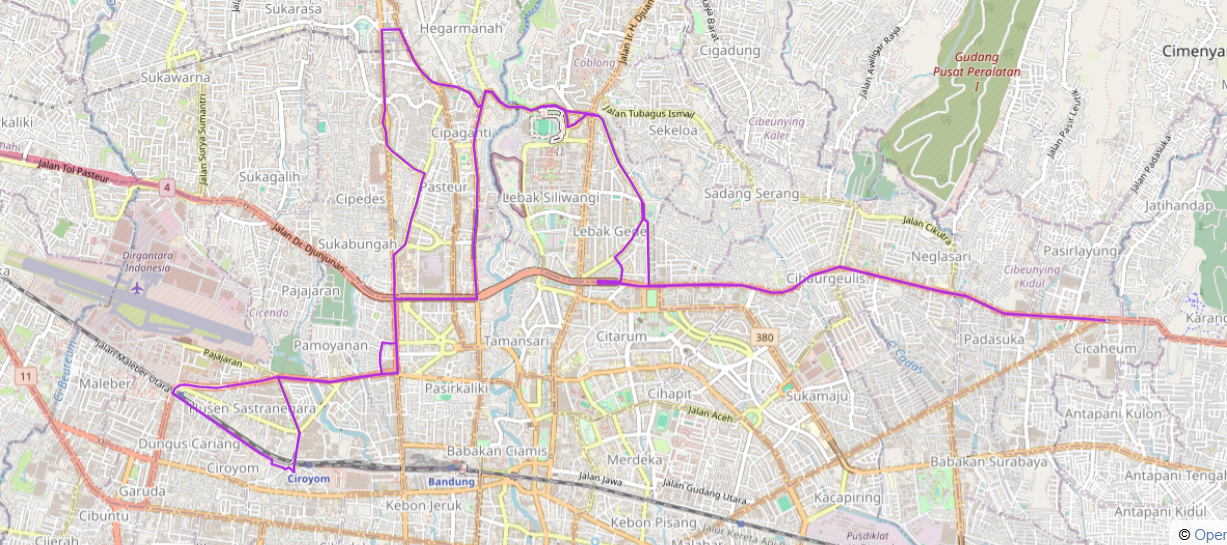
\includegraphics[width=1\textwidth]{pemodelan-graf}  
    \caption{Rute Ciroyom – Cicaheum}
    \label{fig:pemodelangraf} 
\end{figure}
\noindent
Pada bagian ini, akan dilakukan analisis mengenai bagaimana rute-rute yang terdapat dalam tabel \texttt{tracks} pada database dapt dimodelkan menjadi sebuah graf oleh NewMenjangan. Gambar \ref{fig:pemodelangraf} merupakan visualisasi GIS (\textit{Geographic Information System}) dari rute angkot cicaheum-ciroyom.

Pada saat NewMenjangan dijalankan data dari tabel \texttt{tracks} akan diambil dengan menggunakan method \texttt{pull()} yang terdapat pada kelas \texttt{DataPuller} \ref{subss:datapuller} dalam format LineString \ref{subs:linestring}. Kemudian data yang telah berhasil diambil akan diubah formatnya menjadi bentuk array \texttt{LngLatAlt} (\textit{longitude} dan \textit{latitude}) menggunakan method \texttt{lineStringToLngLatArray} yang juga terdapat pada kelas \texttt{DataPuller} \ref{subss:datapuller}. Dari Titik-titik yang terdapat pada array \texttt{LngLatAlt} akan dimodelkan menjadi graf dengan menjadikan setiap titik menjadi sebuah \textit{node} dan akan dihubungkan dengan \textit{edge} antara nodenya, selain itu juga apabila ada dua titik dari rute angkot berbeda atau disebut juga \textit{transferNode} yang jaraknya dibawah dari konstanta yang telah ditentukan, maka akan dibuatkan juga sebuah \textit{edge} untuk menghubungkannya. Pemodelan graf tersebut menggunakan method-method pada kelas \texttt{Worker} \ref{subss:worker} yang juga memanfaatkan \textit{method-method} pada kelas \texttt{Graph} \ref{subss:graph}, \texttt{GraphNode} \ref{subss:graphnode}, \texttt{LatLon} \ref{subss:latlon}, dan \texttt{Track} \ref{subss:track}.

\section{Analisis Sistem Usulan}
Analisis ini dilakukan terhadap sistem usulan yang bertujuan untuk meningkatkan fleksibilitas dan efisiensi dalam proses pencarian rute terpendek pada perangkat lunak KIRI. Sistem yang diusulkan mengadopsi \textit{strategy pattern} sebagai pola desain untuk memisahkan logika implementasi algoritma \textit{shortest path}, sehingga memungkinkan penggantian atau penambahan algoritma dengan lebih mudah. Selain algoritma Dijkstra yang telah diterapkan pada sistem saat ini, sistem usulan juga mengimplementasikan dua algoritma tambahan, yaitu Floyd-Warshall dan A-Star. Penambahan kedua algoritma ini bertujuan untuk memperluas cakupan kebutuhan kasus penggunaan yang beragam, di mana Floyd-Warshall cocok untuk penghitungan semua pasangan titik, sedangkan A-Star menawarkan efisiensi untuk pencarian rute dengan heuristik tertentu. Dengan demikian, sistem usulan diharapkan dapat mengatasi keterbatasan sistem yang ada, yang saat ini hanya menggunakan satu algoritma dan belum mengadopsi pola desain modular seperti \textit{strategy pattern}.

\subsection{Implementasi Strategy Pattern}
Implementasi \textit{strategy pattern} pada NewMenjangan bertujuan untuk memberikan KIRI kebebasan untuk memilih dan menentukan strategi yang akan dipilih, dalam kasus ini adalah algoritma \textit{shortest path}. Selain itu, juga memberikan fleksibilitas yang tinggi serta memberikan kemudahan dalam menambahkan atau mengganti algoritma ketika proses pengembangan perangkat lunak, seperti yang telah dijelaskan pada subbab \ref{sec:designdanstrategypattern}.
\begin{figure}[h] 
    \centering  
    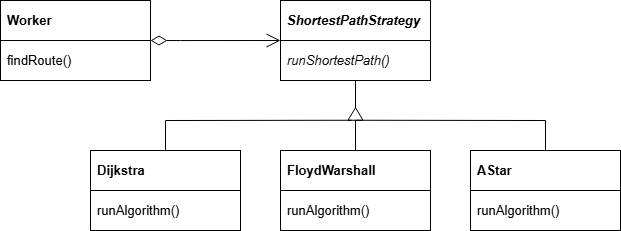
\includegraphics[width=1\textwidth]{Struktur-SP2}  
    \caption{Struktur Strategy Pattern}
    \label{fig:struktursp2} 
\end{figure}

Gambar \ref{fig:struktursp2} menunjukkan struktur \textit{strategy pattern} yang dirancang untuk implementasi yang akan dilakukan dalam tugas akhir ini. Gambar \ref{fig:struktursp2} menjelaskan bagaimana \textit{strategy pattern} diimplementasikan dengan algoritma Dijkstra, A-Star, dan Floyd-Warshall sebagai \textit{concrete strategy}. Kemudian, kelas \texttt{ShortestPathAlgorithm} sebagai \textit{Strategy} dan kelas Worker sebagai \textit{Context}.
\newpage
\subsection{Implementasi Algoritma A-Star dan Algoritma Floyd-Warshall}
Sistem usulan dirancang untuk meningkatkan performa dan fleksibilitas dalam penentuan rute terpendek dengan mengimplementasikan algoritma A-Star dan Floyd-Warshall. Pada sistem saat ini, hanya algoritma Dijkstra yang telah diimplementasikan. Algoritma A-Star dan Floyd-Warshall juga sama seperti algoritma Dijkstra yang termasuk algoritma \textit{shortest path} yang digunakan untuk mencari rute terdekat, seperti yang sudah dijelaskan pada subbab \ref{a*} dan \ref{floydwarshall}. Perubahan akan dilakukan pada NewMenjangan untuk mengimplementasikan algoritma A-Star dan Floyd-Warshall, yaitu dengan menambahkan 2 kelas java baru dengan nama FloydWarshall.java dan AStar.java.